%%%%%%%%%%%%%%%%%%%%%%%%%%%%%%%%%%%%%%%%%
% Formal Text-Rich Title Page 
% LaTeX Template
% Version 1.0 (27/12/12)
%
% This template has been downloaded from:
% http://www.LaTeXTemplates.com
%
% Original author:
% Peter Wilson (herries.press@earthlink.net)
%
% License:
% CC BY-NC-SA 3.0 (http://creativecommons.org/licenses/by-nc-sa/3.0/)
% 
% Instructions for using this template:
% This title page compiles as is. If you wish to include this title page in 
% another document, you will need to copy everything before 
% \begin{document} into the preamble of your document. The title page is
% then included using \titleGP within your document.
%
%%%%%%%%%%%%%%%%%%%%%%%%%%%%%%%%%%%%%%%%%

%----------------------------------------------------------------------------------------
%  PACKAGES AND OTHER DOCUMENT CONFIGURATIONS
%----------------------------------------------------------------------------------------

\documentclass{book}

\newcommand*{\plogo}{\fbox{$\mathcal{PL}$}} % Generic publisher logo
\usepackage{geometry}
\usepackage{url}

%----------------------------------------------------------------------------------------
%	TITLE PAGE
%----------------------------------------------------------------------------------------


\newcommand*{\titleGP}{\begingroup % Create the command for including the title page in the document
\centering % Center all text
\vspace*{\baselineskip} % White space at the top of the page

\rule{\textwidth}{1.6pt}\vspace*{-\baselineskip}\vspace*{2pt} % Thick horizontal line
\rule{\textwidth}{0.4pt}\\[\baselineskip] % Thin horizontal line

{\Huge CONTROL FLU \\[0.4\baselineskip]  
DATA INSIGHTS}\\[0.4\baselineskip] % Title

\rule{\textwidth}{0.4pt}\vspace*{-\baselineskip}\vspace{3.2pt} % Thin horizontal line
\rule{\textwidth}{1.6pt}\\[\baselineskip] % Thick horizontal line

\scshape % Small caps
\Large{Report 1 of 3}  \\[\baselineskip] % Tagline(s) or further description

\begin{Large}
Estimating county-wide pediatric influenza immunization uptake\par % Location and year
\end{Large}
\vspace*{2\baselineskip} % Whitespace between location/year and editors

 \\[\baselineskip]
{\large DISEASE CONTROL UNIT\par} % Editor list
{\itshape Joe Brew\par} % Editor affiliation

\vfill % Whitespace between editor names and publisher logo

 \\[0.3\baselineskip] % Publisher logo
{\scshape December 2014} \\[0.3\baselineskip] % Year published
{\large joseph.brew@flhealth.gov}\par % Publisher

\endgroup}

%----------------------------------------------------------------------------------------
%	BLANK DOCUMENT
%----------------------------------------------------------------------------------------


\usepackage{Sweave}
\begin{document} 

\pagestyle{empty} % Removes page numbers

\titleGP % This command includes the title page
\Sconcordance{concordance:county_wide_imm_rate_by_age_group.tex:county_wide_imm_rate_by_age_group.Rnw:%
1 75 1 1 0 7 1 1 121 26 1 1 3 1 2 2 1 1 3 1 2 2 1 1 3 1 2 2 1 1 3 1 2 2 %
1}




\newgeometry{margin = 3cm}
\section*{Context}
This is the first in a three-part program evaluation of the "Control Flu"program using a combination of Alachua County Public Schools, Florida Shots, and Census data.  This report deals with county-wide pediatric immunization rates from 2011-12 to 2013-14.  The second report (mid-December 2014) will cover immunization uptake among Alachua's public school students, with a focus on assessing likelihood to immunize by sociodemographic traits (so as to assist with program targeting and identification of groups at greatest risk).  The final report (January 2015) will cover the program's impact on absenteeism.  

\section*{Summary}
School-specific immunization rates are helpful in determining "Control Flu" program performance, and for tracking changes over time.  However, school-specific rates (and changes over time) do not necessarily reflect community-wide immunization, since many families choose to get immunized outside of the "Control Flu" program. Additionally, given that (a) a number of schools do not participate in the "Control Flu" program and (b) a number of Alachua county youth residents are not enrolled in traditional schools (ie, homeschooled, institutionalized, etc.), a broader view is needed to fully understand pediatric immunization over time. \\

In order to provide this broader view, immunization was analyzed using Florida Shots data (instead of only "Control Flu" records).   Though we have some data going through the beginning of the 2014-15 season, these are incomplete (and therefore not included in this analysis).

\section*{Details}
Census data was used to provide a "denominator" by which yearly county-wide immunization rates could be calculated. This has the advantage of including young people who do not attend schools which participate in the "Control Flu" program.  However, age groups ("Pre-K", "Elementary", "Middle", or "High") were \emph{estimated} based on a child's age at the date of immunization, and are therefore not exact. For example, "Pre-K" includes all children younger than age 5 (which partially explains the very low rates).

\section*{Understanding the charts}
 The charts on pages 3 and 4 show (a) the overall age-specific immunization rates and numbers (top of bar), (b) the number and percentage of immunizations administered by the County Health Department (CHD, blue), and (c) the number and percentage of immunizations administered by private practitioners (orange).
 
 \section*{Trends and patterns}
 With the exception of the Pre-K age group (for whom the data are least reliable, given the age cut-offs), all age groups have seen both absolute and relative growth in immunization in the last 3 years.  Of particular note is a slightly greater than expected jump in privately-administered vaccinations in the 2013-14 school year.  The reasons for this are unknown, but could be related to local media attention paid to the severity of the flu season in Decmeber 2013 and January 2014.  
 


% \section*{Data and code}
% Florida Shots data are not available for public disclosure.  However, census data and the code used for tabulations and graphics can be viewed at \url{https://github.com/joebrew/fdoh/tree/master/public/ab_chd_private}.



\begin{center}
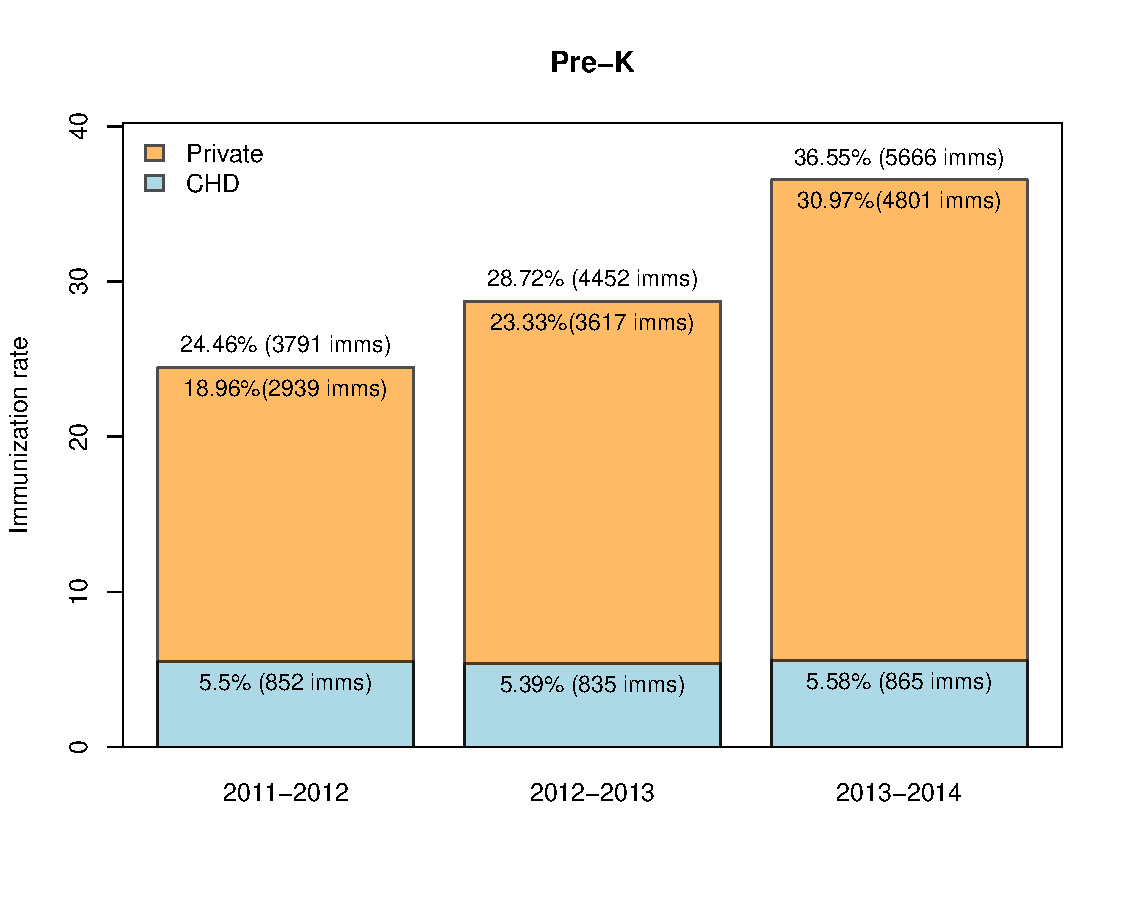
\includegraphics{county_wide_imm_rate_by_age_group-002}
\end{center}

\begin{center}
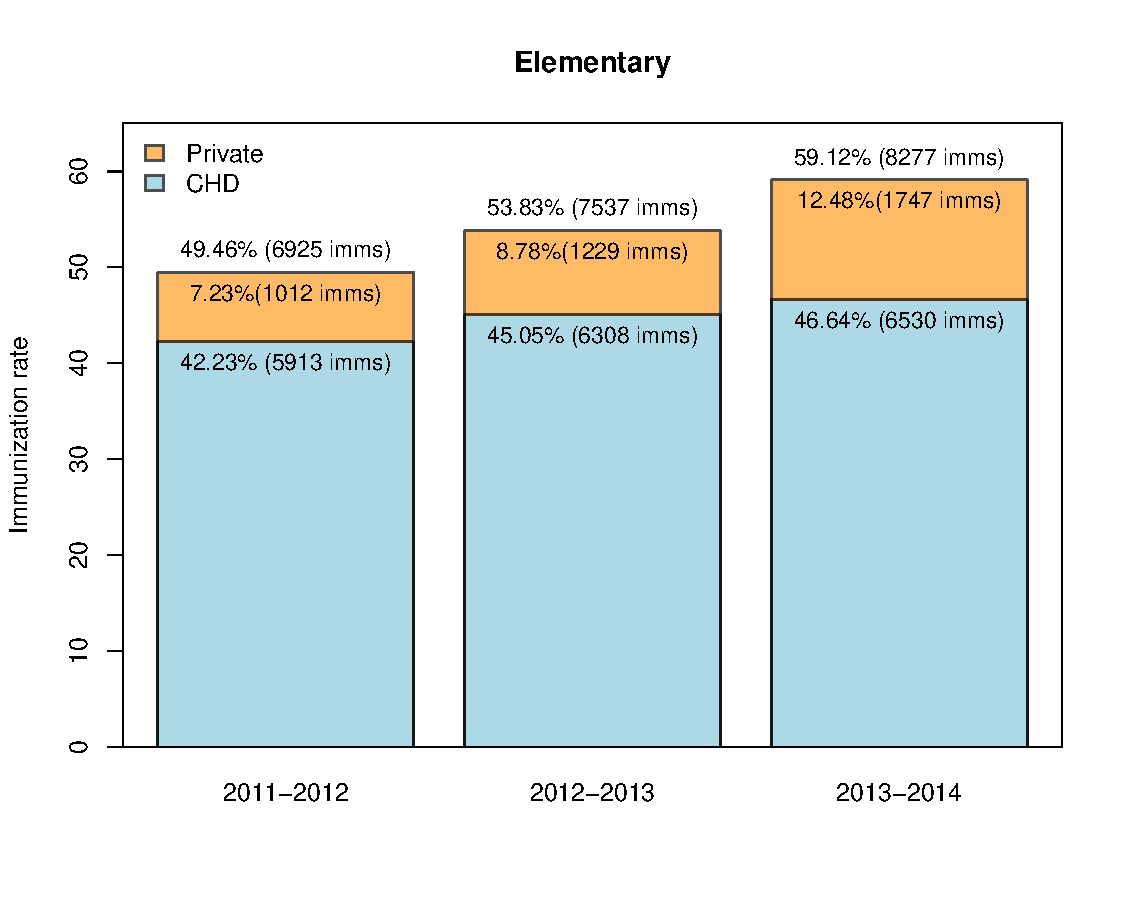
\includegraphics{county_wide_imm_rate_by_age_group-003}
\end{center}

\begin{center}
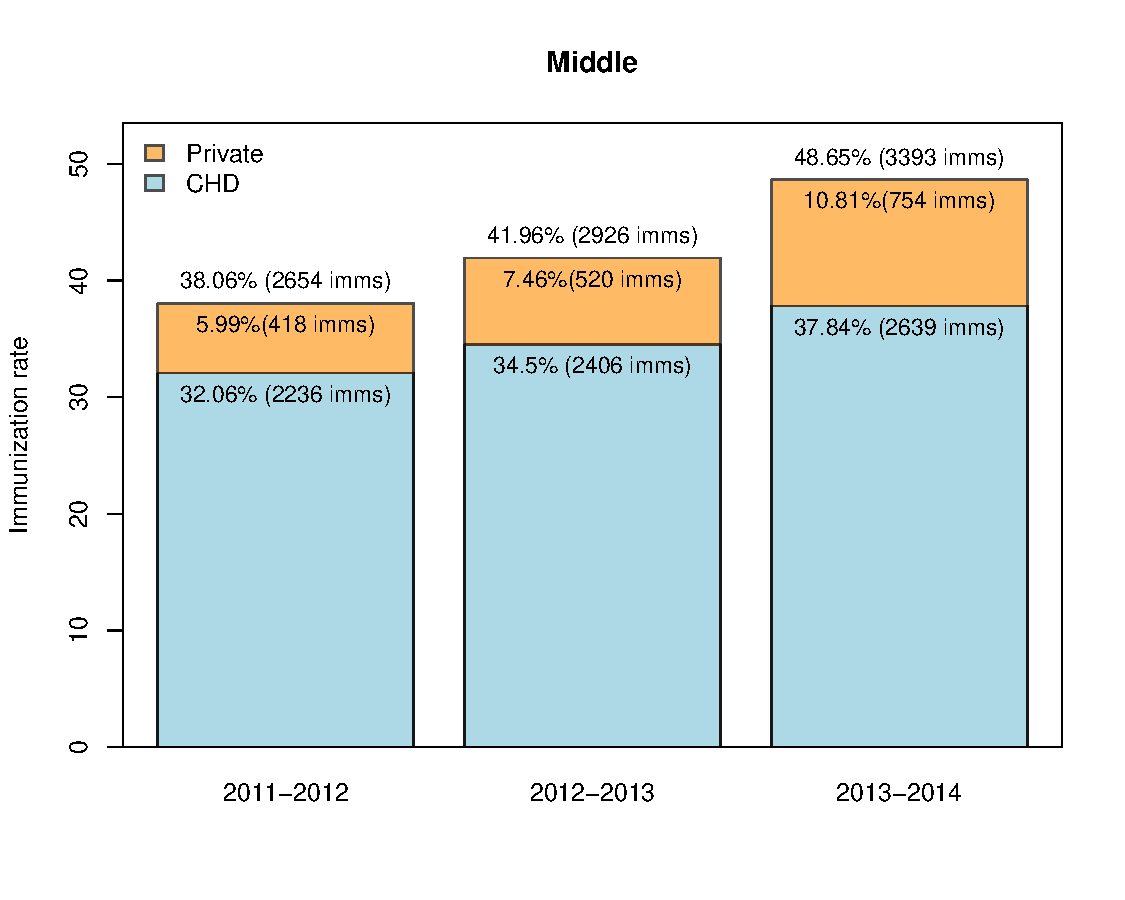
\includegraphics{county_wide_imm_rate_by_age_group-004}
\end{center}

\begin{center}
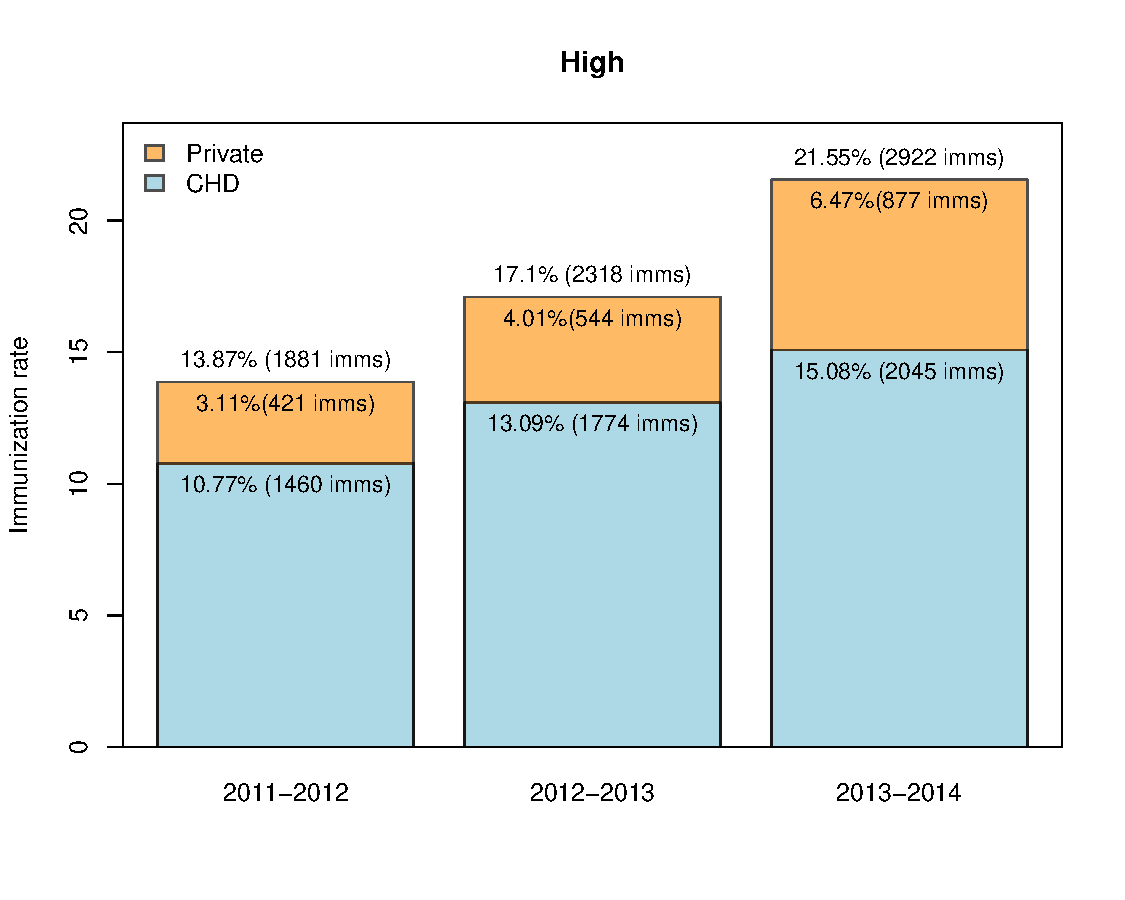
\includegraphics{county_wide_imm_rate_by_age_group-005}
\end{center}

\end{document}
